\documentclass[10pt,aspectratio=169]{beamer}
\usetheme{metropolis}
\usepackage{appendixnumberbeamer}
\usepackage{booktabs}
\usepackage{graphicx}
\usepackage{tikz}
\usepackage{amsmath}
\usepackage{xcolor}

% Define NHS colors
\definecolor{nhsblue}{RGB}{0,94,184}
\definecolor{nhsdarkblue}{RGB}{0,48,135}
\definecolor{nhsgreen}{RGB}{0,177,64}
\definecolor{nhsred}{RGB}{218,41,28}

% Set theme colors
\setbeamercolor{frametitle}{bg=nhsblue,fg=white}
\setbeamercolor{progress bar}{fg=nhsgreen}
\setbeamercolor{title separator}{fg=nhsblue}
\setbeamercolor{alerted text}{fg=nhsred}

\metroset{progressbar=frametitle,sectionpage=progressbar,numbering=fraction}

\title{Agent-Based Simulation for Neovascular AMD Treatment Planning}
\subtitle{Optimizing Anti-VEGF Therapy Protocols in the NHS}
\author{Luke Herbert\\Consultant Ophthalmologist}
\institute{Surrey and Sussex Healthcare NHS Trust}
\date{24th June 2025}

\begin{document}

\section{Why Model?}

\begin{frame}{The Need for Modeling}
\begin{columns}[T]
\column{0.5\textwidth}
\textbf{Current Challenges:}
\begin{itemize}
    \item Treatment controversies
    \item Limited real-world data
    \item Complex patient pathways
    \item Resource constraints
\end{itemize}

\column{0.5\textwidth}
\textbf{Modeling Benefits:}
\begin{itemize}
    \item Explore treatment strategies
    \item Clarify outcome measures
    \item Predict resource needs
    \item Evidence-based decisions
\end{itemize}
\end{columns}
\end{frame}

\begin{frame}{Two Modeling Approaches}
\begin{columns}[T]
\column{0.5\textwidth}
\textbf{Simple Approach (NHS England):}
\begin{itemize}
    \item Excel spreadsheet
    \item "Best guess" parameters
    \item Average patient behavior
    \item Quick but limited insights
\end{itemize}

\column{0.5\textwidth}
\textbf{Our Approach (Agent-Based):}
\begin{itemize}
    \item Individual patient simulation
    \item Build from known parameters
    \item Probabilistic events
    \item Rich, detailed insights
\end{itemize}
\end{columns}

\vspace{0.5cm}
\centering

\begin{tikzpicture}
    \node[draw,nhsblue,thick,minimum width=3cm] (excel) at (0,0) {Excel Model};
    \node[draw,nhsgreen,thick,minimum width=3cm] (agent) at (7,0) {Agent-Based Model};
    \draw[->,thick] (excel.east) -- node[above] {Evolution} (agent.west);
\end{tikzpicture}
\end{frame}

\begin{frame}{Real-World Complexity in Our Simulation}
\begin{alertblock}{Model Comparison}
\begin{columns}[T]
\column{0.5\textwidth}
\textbf{Simple Models Assume:}
\begin{itemize}
    \item All patients start with same vision
    \item Perfect treatment adherence
    \item No appointment delays
    \item Uniform response to treatment
\end{itemize}

\column{0.5\textwidth}
\textbf{Our Simulation Includes:}
\begin{itemize}
    \item \alert{Vision distribution at baseline}
    \item \alert{Real discontinuation patterns}
    \item \alert{Treatment gaps and delays}
    \item Individual patient trajectories
\end{itemize}
\end{columns}
\end{alertblock}

\begin{block}{Why This Matters}
\begin{itemize}
    \item Captures NHS capacity constraints
    \item Models actual patient populations
    \item Predicts realistic outcomes
    \item Enables better resource planning
\end{itemize}
\end{block}

\centering
\textbf{Result: Evidence-based insights, not theoretical averages}
\end{frame}

\section{Our Solution}

\begin{frame}{Application Architecture}
\centering
\textbf{Four Key Modules:}

\vspace{0.5cm}
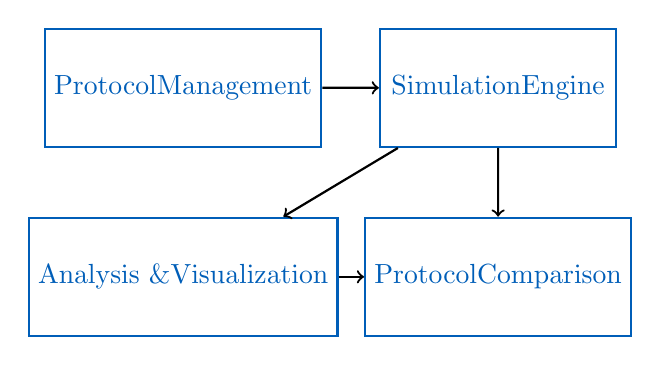
\begin{tikzpicture}[scale=0.8]
    \node[draw,nhsblue,thick,minimum width=3cm,minimum height=1.5cm] (proto) at (0,3) {Protocol\\Management};
    \node[draw,nhsblue,thick,minimum width=3cm,minimum height=1.5cm] (sim) at (5,3) {Simulation\\Engine};
    \node[draw,nhsblue,thick,minimum width=3cm,minimum height=1.5cm] (analysis) at (0,0) {Analysis \&\\Visualization};
    \node[draw,nhsblue,thick,minimum width=3cm,minimum height=1.5cm] (compare) at (5,0) {Protocol\\Comparison};
    
    \draw[->,thick] (proto) -- (sim);
    \draw[->,thick] (sim) -- (analysis);
    \draw[->,thick] (sim) -- (compare);
    \draw[->,thick] (analysis) -- (compare);
\end{tikzpicture}

\vspace{0.5cm}
\alert{Next: Live demonstration of the application}
\end{frame}

% Placeholder for screen recording section
\begin{frame}{Live Demonstration}
\centering
\Large
[Switch to Screen Recording]

\normalsize
\vspace{1cm}
Demonstration includes:
\begin{itemize}
    \item Loading treatment protocols
    \item Running 1000-patient simulation
    \item Exploring patient journeys
    \item Visualizing population outcomes
    \item Comparing different protocols
\end{itemize}
\end{frame}

\section{Key Insights}

\begin{frame}{What We've Learned}
\begin{columns}[T]
\column{0.5\textwidth}
\textbf{Model Reveals:}
\begin{itemize}
    \item Treatment pattern impacts
    \item Resource utilization peaks
    \item Patient outcome distributions
    \item Protocol efficiency metrics
\end{itemize}

\column{0.5\textwidth}
\textbf{Enables:}
\begin{itemize}
    \item Evidence-based protocols
    \item Capacity planning
    \item Cost-effectiveness analysis
    \item Commissioning decisions
\end{itemize}
\end{columns}

\vspace{0.5cm}
\begin{alertblock}{Future Development}
Cost calculator module in development for full economic analysis
\end{alertblock}
\end{frame}

\begin{frame}{Thank You}
\centering
\Large
Questions?

\vspace{1cm}
\normalsize
\textbf{Contact:}\\
your.email@nhs.net

\vspace{0.5cm}
\textbf{Project Repository:}\\
\url{https://github.com/lh/vegf-1} \\
\textbf{Application:}\\
\url{https://vegf-1.streamlit.app}

\vspace{0.5cm}
\textbf{Acknowledgments:}\\
HSMA Team | NHS England | Trust Leadership
\end{frame}

\end{document}